\documentclass[11pt]{article}

%%% XeLaTeX Font Definitions

\usepackage{titlesec}
\usepackage{titling}
\usepackage{xunicode}
\usepackage{fontspec,xltxtra,xunicode}

\defaultfontfeatures{Mapping=tex-text}

% Uncomment below to change default features 
%\setromanfont[Mapping=tex-text]{Hoefler Text}
%\setsansfont[Scale=MatchLowercase,Mapping=tex-text]{Gill Sans}
%\setmonofont[Scale=MatchLowercase]{Andale Mono}

% Specify different font for section headings
\newfontfamily\headingfont[]{Lucida Grande Bold}
\newfontfamily\titlefont[]{Optima}

\titleformat*{\section}{\Large\headingfont}
\titleformat*{\subsection}{\large\headingfont}
\titleformat*{\subsubsection}{\large\headingfont}
\renewcommand{\maketitlehooka}{\titlefont}

%%% Remove the "abstract" word before the abstract

\usepackage{abstract}
\renewcommand{\abstractname}{}    % clear the title
\renewcommand{\absnamepos}{empty} % originally center

%%% Actual Preamble

%\headheight=8pt
%\topmargin=3pt
%\textheight=624pt
%\textwidth=432pt
%\oddsidemargin=18pt
%\evensidemargin=18pt

\usepackage{amsmath}
\usepackage{amsfonts}
\usepackage{amssymb}
\usepackage{amsthm}
\usepackage{comment}
\usepackage{epsfig}
\usepackage{psfrag}
%\usepackage{sseq} (if you need to draw spectral sequences, please use this package, available at http://wwwmath.uni-muenster.de/u/tbauer/)
\usepackage{mathrsfs}
\usepackage{amscd}
\usepackage[all]{xy}
\usepackage{rotating}
\usepackage{lscape}
\usepackage{amsbsy}
\usepackage{verbatim}
\usepackage{moreverb}
\usepackage{mathdots}
\usepackage{setspace}
%\usepackage{eucal}
\usepackage{hyperref}
\usepackage{pgfplots}%http://www.ctan.org/pkg/pgfplots

\usepackage{listings}
\usepackage[margin=1in]{geometry}
\pagestyle{plain}
\theoremstyle{definition}
\newtheorem{theorem}{Theorem}%[section]
\newtheorem{prop}[theorem]{Proposition}
\newtheorem{lemma}[theorem]{Lemma}
\newtheorem{corollary}[theorem]{Corollary}
%\theoremstyle{definition}
\newtheorem{definition}[theorem]{Definition}
\newtheorem{notation}[theorem]{Notation}
\newtheorem{summary}[theorem]{Summary}
\newtheorem{note}[theorem]{Note}
\newtheorem{construction}[theorem]{Construction}
%\theoremstyle{remark}
\newtheorem{remark}[theorem]{Remark}
\newtheorem{example}[theorem]{Example}
\newtheorem{question}[theorem]{Question}
\DeclareMathOperator{\Aut}{Aut}
\DeclareMathOperator{\coeq}{coeq}
\DeclareMathOperator{\colim}{colim}
\DeclareMathOperator{\cone}{cone}
\DeclareMathOperator{\Der}{Der}
\DeclareMathOperator{\Ext}{Ext}
\DeclareMathOperator{\hocolim}{hocolim}
\DeclareMathOperator{\holim}{holim}
\DeclareMathOperator{\Hom}{Hom}
\DeclareMathOperator{\Iso}{Iso}
\DeclareMathOperator{\Map}{Map}
\DeclareMathOperator{\Tot}{Tot}
\DeclareMathOperator{\Tor}{Tor}
\DeclareMathOperator{\Spec}{Spec}
\newcommand{\TMF}{\mathit{TMF}}
\newcommand{\tmf}{\mathit{tmf}}
\newcommand{\Mell}{\mathcal M_{\mathit{ell}}}
\newcommand{\Mord}{\mathcal M_{\mathit{ell}}^{\mathit{ord}}}
\newcommand{\Mss}{\mathcal M_{\mathit{ell}}^{\mathit{ss}}}
\newcommand{\Mbar}{\overline{\mathcal M}_{\mathit{ell}}}
\newcommand{\Mfg}{\mathcal M_{\mathit{FGL}}}
\newcommand{\MU}{\mathit{MU}}
\newcommand{\MP}{\mathit{MP}}
\newcommand{\Lk}{L_{K(n)}}
\newcommand{\Lone}{L_{K(1)}}
\newcommand{\Ltwo}{L_{K(2)}}
\newcommand{\Sp}{\mathbf{Sp}}
\newcommand{\Eoo}{E_\infty}
\newcommand{\Aoo}{A_\infty}
\newcommand{\CP}{\mathbb{CP}^\infty}
\newcommand{\GL}{\mathit{GL}}
\newcommand{\gl}{\mathit{gl}}
\newcommand{\nn}{\nonumber}
\newcommand{\nid}{\noindent}
\newcommand{\ra}{\rightarrow}
\newcommand{\la}{\leftarrow}
\newcommand{\xra}{\xrightarrow}
\newcommand{\xla}{\xleftarrow}
\newcommand{\weq}{\xrightarrow{\sim}}
\newcommand{\cofib}{\rightarrowtail}
\newcommand{\fib}{\twoheadrightarrow}
 \newcommand{\xhdr}[1]{\vspace{2mm}\noindent{{\bf #1.}}}

\def\llarrow{   \hspace{.05cm}\mbox{\,\put(0,-2){$\leftarrow$}\put(0,2){$\leftarrow$}\hspace{.45cm}}}
\def\rrarrow{   \hspace{.05cm}\mbox{\,\put(0,-2){$\rightarrow$}\put(0,2){$\rightarrow$}\hspace{.45cm}}}
\def\lllarrow{  \hspace{.05cm}\mbox{\,\put(0,-3){$\leftarrow$}\put(0,1){$\leftarrow$}\put(0,5){$\leftarrow$}\hspace{.45cm}}}
\def\rrrarrow{  \hspace{.05cm}\mbox{\,\put(0,-3){$\rightarrow$}\put(0,1){$\rightarrow$}\put(0,5){$\rightarrow$}\hspace{.45cm}}}
\def\cA{\mathcal A}\def\cB{\mathcal B}\def\cc{\mathbf C}\def\cd{\mathbf D}
\def\ce{\mathcal E}\def\cf{\mathcal F}\def\cG{\mathcal G}\def\cH{\mathcal H}
\def\cI{\mathcal I}\def\cJ{\mathcal J}\def\cK{\mathcal K}\def\cL{\mathcal L}
\def\cM{\mathbf M}\def\cN{\mathcal N}\def\cO{\mathbf O}\def\cP{\mathcal P}
\def\cQ{\mathcal Q}\def\cR{\mathcal R}\def\cS{\mathcal S}\def\cT{\mathcal T}
\def\cU{\mathcal U}\def\cV{\mathcal V}\def\cW{\mathcal W}\def\cX{\mathcal X}
\def\cY{\mathcal Y}\def\cZ{\mathcal Z}
\def\AA{\mathbb A}\def\BB{\mathbb B}\def\CC{\mathbb C}\def\DD{\mathbb D}
\def\EE{\mathbb E}\def\FF{\mathbb F}\def\GG{\mathbb G}\def\HH{\mathbb H}
\def\II{\mathbb I}\def\JJ{\mathbb J}\def\KK{\mathbb K}\def\LL{\mathbb L}
\def\MM{\mathbb M}\def\NN{\mathbb N}\def\OO{\mathbb O}\def\PP{\mathbb P}
\def\QQ{\mathbb Q}\def\RR{\mathbb R}\def\SS{\mathbb S}\def\TT{\mathbb T}
\def\UU{\mathbb U}\def\VV{\mathbb V}\def\WW{\mathbb W}\def\XX{\mathbb X}
\def\YY{\mathbb Y}\def\ZZ{\mathbb Z}

\newcommand{\MFGL}{\mathcal M_{\mathit{FGL}}}
\newcommand{\calO}{{\mathcal O}}
\newcommand{\calC}{{\mathcal C}}
\newcommand{\set}{{\mathrm{Set}}}
\newcommand{\Deltab}{{\mathbf \Delta}}
\newcommand{\spet}{\mathrm{Spec}^\mathrm{\acute{e}t}}
\newcommand{\Z}{\mathbb Z}
\DeclareMathOperator{\Spf}{Spf}
\setlength\parindent{0pt}

\begin{document}
\title{\headingfont{Information Theory}}
\author{Manan Shah\\ \texttt{manan.shah.777@gmail.com} \\ The Harker School}
\maketitle
\begin{abstract}
This document contains lecture notes from Harker's Advanced Topics in Mathematics class in Information Theory, Parts I and II. These notes were taken using TeXShop and \LaTeX2$\epsilon$ and will be updated for each class. 
\end{abstract}
\tableofcontents
\newpage

%% Notes start here

\section{August 22, 2016}
\subsection{Class Overview}
\begin{figure}[h]
\centering
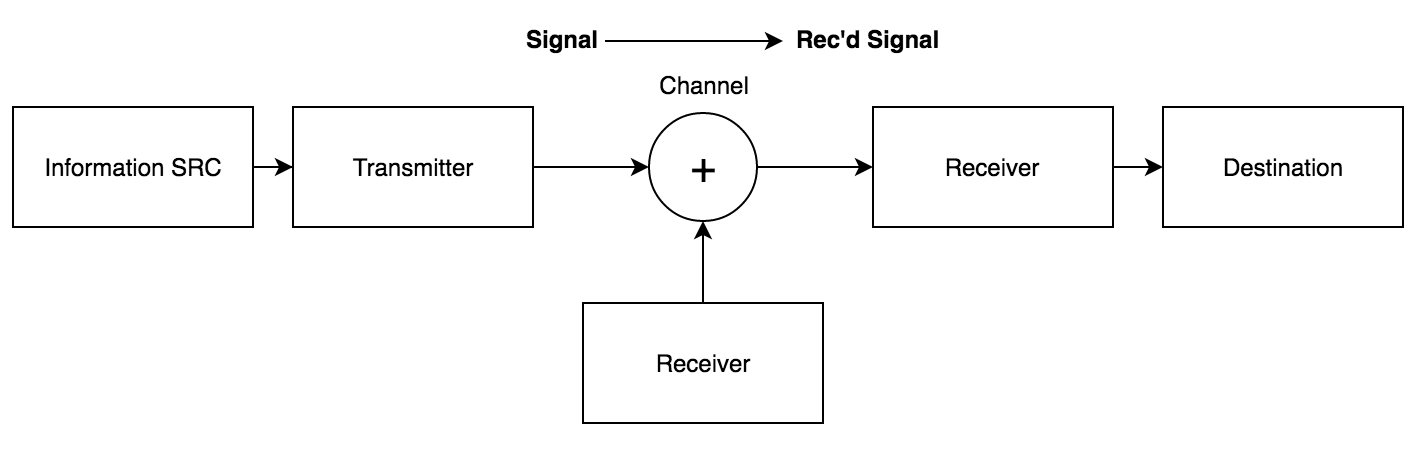
\includegraphics[scale=0.5]{pipeline}
\end{figure}
Information may be conveyed in multiple ways; for example, by a person talking, a video, or pictures. Our goal is to model this kind of information as a system with one output and no input. The information is therefore a box that emits output probabilistically, and we will therefore be spending 1-2 weeks on probability, specifically regarding distribution functions and expectation. This is illustrated in the ``information source'' box---the job of the information source is to \textbf{provide the signal}. 

We will next define the compression problem; having obtained numbers as a stream, the problem is to remove the redundancy in a stream. In particular, we will discuss both lossless and lossy compression. One of the most critical ideas in this course is that of entropy, and we will define the concept (in general, a notion of how much information is originating from the source). We will also discuss the sensibility of such a definition and potentially expand upon it. An overarching concept here will be our definition of the performance of a compression algorithm via the source compression theorem and the boundedness of compression algorithms. This is illustrated in the ``transmitter'' box---the job of the transmitter is to \textbf{remove all redundancy}.

We will subsequently discuss the channel circle, which we will model with conditional probability distribution functions (PDFs). The output of this box, the receiver signal, is input to the receiver box, which has the job of \textbf{reconstruction of the signal and the noise}; this is known as the coding problem. Much like the compression problem of the source, the channel has the capacity problem (how much information can be transmitted?). And similar to the compression theorem, we will discuss the channel coding theorem, which will help us determine which parts of a code will require more redundancy for transmission. 

We will finally discuss Shannon's theorem, in which he states that a communication with no loss and arbitrary cost (due to a constraint on the amount of bandwith, power, etc.) is possible if the entropy of the source $H$ is less than the capacity of the channel $C$. In our course, we will first discuss the pipeline for lossless compression and then move to lossy compression.

\section{August 24, 2016}
Knowing what a random variable is and what it means is important for the source to transmitter relationship. 
\subsection{Random Variables}
\definition A random variable is a real-valued function of the outcome of an experiment. By definition, it is not deterministic.
\notation We will represent random variables with capital letters (for example, $X, Y, Z$).
\example[What are Random Variables?] (a) A coin is tossed ten times. Determine the number of heads obtained from the coin toss. The number of heads is the random variable in this case. (b) Given two rolls of die, identify their sum (a random variable) and the second roll raised to the fifth power (another random variable). (c) The time to transmit a message, the delay with which a message is received, and the number of errors in a message are both themselves random variables. \\

Two types of random variables exist; discrete variables and continuous variables. 
\definition[Discrete RV] A discrete random variable is one that has a finite set of outcomes (or is countably infinite), and has a probability associated with each outcome. 
\definition[Continuous RV] A continuous random variable is one that has a non-finite, uncountable set of outcomes. 

\example Define the function 
\begin{equation*}
sgn(a) = \begin{cases}
1 &a > 0\\
0 & a = 0 \\
-1 & a < 0
\end{cases}
\end{equation*}
The variable $a$ is a continuous random variable, while $sgn(a)$ is a discrete function (with outputs $\in \{1, 0, -1\}$)
\subsubsection{Probability Mass Function (pmf)}
Probability mass functions are functions of a discrete random variable, describing all instances of a random variable occurring and its associated probabilities. Define $X$ as a random variable, and write $P(X = x)$ as $p_X(x)$. Then $\sum_x p_X(x) = 1$. Consider two tosses of a coin, letting $X$ equal the number of heads obtained. We therefore have 
\begin{equation*}
p_X(x) = \begin{cases}
1/4 & x =0\\
1/2 & x=1\\
1/4 & x=2 \\
\end{cases}
\end{equation*}
note that $p_X(x)$ is clearly a discrete function that takes on values $x \in \{0, 1, 2 \}$ with respective output probabilities. 
\subsubsection{Probability Densify Function (pdf)}
%\begin{figure*}[h]
%\centering
%    \begin{tikzpicture}
%    \path[draw](0,0)--(0,5);
%    \path[draw](0,0)--(5,0);
%     \path[draw] (0,0) -- (2,2) -- (4,0);
%    \end{tikzpicture}
%\end{figure*}
Probability density functions are functions of a continuous random variable. Define $X$ as a random variable. In this case, the expression $P(X = x)$ is meaningless (in fact, it is defined as 0). The probability of a range of values from $x = a$ to $x = b$ is more relevant; in particular, $\int_{-\infty}^{\infty}p_X(x) = 1$. 

\example Edgar's driving time to school is between 15 and 20 minutes if it is sunny and between 20 and 25 minutes if it is a rainy day. Assume a day is sunny with $2/3$ probability and rainy with $1/3$ probability. Construct the respective PDF. \\

The PDF construction is quite simple; remember that $\int_{-\infty}^{\infty}p_X(x) = 1$. 
\begin{equation*}
p_X(x) = \begin{cases}
2/15 & 15 \leq x \leq 20\\
1/15 & 20 \leq x \leq 25 \\
0 & x \geq 25 \\
\end{cases}
\end{equation*}

\subsubsection{Types of Random Variables}
We will define these distributions in terms of a coin toss. 

\xhdr{Bernoulli (Discrete)} Toss a coin, and it define the probability of heads as $p$. The respective PMF is 
\begin{equation*}
p_X(x) = \begin{cases}
p & x = 1\\
(1-p) & x = 0
\end{cases}
\end{equation*}

\xhdr{Binomial (Discrete)} Toss a coin $N$ times, and define $x$ as the number of heads obtained in $N$ tosses. Let $N = 10$, and define the probability of heads as $p$. Then the respective PMF is 
\begin{equation*}
p_X(x) = \begin{cases}
(1-p)^{10} & x = 0\\
{10 \choose 2}p^2(1-p)^8 & x = 2 \\
\dots & $other values of $ x \in [0, 10] \cup \mathbb{N}
\end{cases}
\end{equation*}

\xhdr{Geometric (Discrete)}  Repeatedly toss a coin until the first ``success.'' This means that we may theoretically have countably infinite $P(X = 1), P(X = 2), P(X = 3), \dots$ output values. Define success to be a head, and the probability of heads as $p$. Then, we have
\begin{equation*}
p_X(x) = \begin{cases}
p & x = 1\\
(1-p)p & x = 2 \\ 
(1-p)^2p & x = 3 \\
\dots & $other values of $ x
\end{cases}
\end{equation*}

\xhdr{Poisson (Discrete)} Instead of tossing a biased coin and counting the number of heads, count the number of times one must replace a biased lightbulb in a time $t$ (with the lightbulb being on or off). 
\end{document}
